% !TEX program = XeLaTeX
% !TEX encoding = UTF-8
\documentclass[UTF8,nofonts]{article}
%{ctexart}


%\setCJKmainfont[BoldFont=FandolSong-Bold.otf,ItalicFont=FandolKai-Regular.otf]{FandolSong-Regular.otf}
%\setCJKsansfont[BoldFont=FandolHei-Bold.otf]{FandolHei-Regular.otf}
%\setCJKmonofont{FandolFang-Regular.otf}

\usepackage{url}
\usepackage{cancel}
\usepackage{xspace}
\usepackage{graphicx}
\usepackage{multicol}
\usepackage{multirow}
\usepackage{subfig}
\usepackage{amsmath}
\usepackage{amssymb}
\usepackage[a4paper, width=186mm, top=18mm, bottom=18mm, includeheadfoot]{geometry}
%\usepackage[a4paper, width=140mm, top=18mm, bottom=22mm, includeheadfoot]{geometry}
\usepackage{booktabs}
\usepackage{array}
\usepackage{verbatim}
\usepackage{caption}
\usepackage{natbib}
\usepackage{booktabs}
\usepackage{float}
\usepackage{pdflscape}
\usepackage{mathtools}
\usepackage[usenames, dvipsnames]{xcolor}
\usepackage{afterpage}
\usepackage{pgf}
\usepackage{tikz}
\usepackage{fontspec}
\usepackage{dirtree}
\usepackage[style=american]{csquotes}
\usepackage{amsfonts}
\usepackage{tikz}
\usepackage{tkz-graph}
\usetikzlibrary{arrows,decorations.pathmorphing,automata,positioning,backgrounds,fit,shapes.symbols,chains,intersections}

\newtheorem{definition}{Definition}[section]
\newtheorem{theorem}{Theorem}[section]
\newtheorem{lemma}{Lemma}
\newtheorem{proof}{Proof} [section]


\usepackage[toc, page, title, titletoc, header]{appendix}
\usepackage{marginnote}
\usepackage{tablefootnote}

%\renewcommand\appendixname{附\ 录}
%\renewcommand\appendixpagename{附\ 录}
%\renewcommand\appendixtocname{附\ 录}
\renewcommand\abstractname{Abstract}


\usepackage{perpage} %the perpage package
\MakePerPage{footnote} %the perpage package command

\usetikzlibrary{shapes.geometric}%
\usepackage{color}
%\usepackage[pages=some, placement=top]{background}
\usepackage{eso-pic}
\usepackage[final]{pdfpages}

%\includepdf[pages=1]{cover}
\hyphenpenalty=750


\title{\textbf{Loopring:}\\\textbf{Un protocole décentralisé d'échange de jetons}}
\author{
  Daniel Wang\\
  \texttt{daniel@loopring.org}\\
  \and
  	Jay Zhou\\
  	\texttt{jay@loopring.org}\\
  	\and
  	Alex Wang\\
  	\texttt{alex@loopring.org}\\
  	\and
  	Matthew Finestone\\
  	\texttt{matt.finestone@gmail.com}\\ 
  \\
  \texttt{https://loopring.org}
 }

\makeatletter
\def\CTEX@section@format{\Large\bfseries}
\makeatother

\makeatletter
\newenvironment{tablehere}
 {\def\@captype{table}}
 {}

\newenvironment{figurehere}
 {\def\@captype{figure}}
 {}
\makeatother



\begin{document}
%\AddToShipoutPicture{\BackgroundPic}
\maketitle

\begin{abstract}
Loopring est un protocole ouvert permettant de créer des échanges décentralisés. Loopring gère des contrats intelligents publiques  pour les échanges et les transactions, avec un groupe hors-chaîne d’acteurs qui agrège et communique les ordres. Le protocole est gratuit, extensible, et sert de standard pour créer les blocs pour les applications décentralisées (dApps) qui incorporent des fonctionnalités d’échange. Son standard inter-opérable facilite les échanges anonymes sans confiance. Une amélioration importante par rapport aux protocoles d'échanges décentralisés actuels est la possibilité de mélanger et d'apparier les ordres avec d'autres ordres dissemblables, évitant ainsi les contraintes liés à l’utilisation de jetons différents et améliorant considérablement la liquidité. Loopring utilise également une solution unique et robuste pour éviter le front-running : la tentative déloyale de soumettre des transactions dans un bloc plus rapidement que le fournisseur d'origine. Loopring est agnostique et peut être déployé sur n'importe quelle chaîne de blocs permettant les fonctionnalités de contrat intelligents. Au moment d'écrire ces lignes, il est utilisable sur Ethereum  \cite{buterin2017ethereum} \cite{wood2014ethereum} et Qtum \cite{dai2017smart} et est en construction pour NEO. \cite{atterlonn2018distributed}
\end{abstract}


\begin{multicols}{2}
\section{Introduction\label{sec:introduction}}

Avec la prolifération des actifs basés sur la chaîne de blocs, la nécessité d'échanger ces actifs entre parties prenantes s'est considérablement accrue. Au fur et à mesure que des milliers de nouveaux jetons sont introduits - y compris pour les actifs traditionnels qui créent leurs propre jetons - ce besoin est amplifié. Qu'il s'agisse d'échanger des jetons pour des motivations commerciales spéculatives ou pour accéder au réseau via leurs jetons utilitaires natifs, la capacité d'échanger un actif cryptographique contre un autre est fondamentale pour l'ensemble de l'écosystème. En effet, il y a une énergie potentielle dans les actifs \cite{desotocapital}, et libérer cette énergie - débloquer le capital - exige non seulement d'affirmer la propriété, ce que les chaînes de blocs ont permis grâce à leur immutabilité, mais aussi la capacité de transférer et de transformer librement ces actifs. 
 
En tant que tel, l'échange sans confiance de jetons (valeur) est un cas d'utilisation convaincant de la technologie des chaînes de blocs. Jusqu'à présent, cependant, les passionnés de cryptographie se sont largement contentés d'échanger des jetons sur des places d'échanges centralisées traditionnelles. Le Protocole Loopring est nécessaire parce que, tout comme Bitcoin \cite{nakamoto2008bitcoin} a mis en avant qu'en ce qui concerne la monnaie électronique de pair à pair, \enquote{les principaux avantages sont perdus si un tiers de confiance est toujours nécessaire pour éviter les doubles dépenses}, il en va de même pour les principaux avantages des actifs décentralisés s'ils doivent passer par des échanges centralisés, et contrôlés.
Échanger des jetons décentralisés sur des places d’échanges centralisés n'a pas de sens d'un point de vue philosophique, car il est alors impossible de maintenir les vertus que ces projets décentralisés épousent. Il existe également de nombreux risques et limites pratiques liés à l'utilisation des places d'échanges centralisées, qui sont décrits ci-dessous. Les échanges décentralisés (DEX) \cite{schuh2015bitshares} \cite{bancor} \cite{bancor} \cite{kyber} ont cherché à résoudre ces problèmes et, dans de nombreux cas, ont réussi à atténuer les risques pour la sécurité en utilisant des chaînes de blocs pour la désintermédiation. Toutefois, comme la capacité des DEX devient cruciale pour la nouvelle économie, il existe une marge de manœuvre importante pour améliorer leurs performances. Loopring vise à fournir des outils modulaires pour ladite infrastructure avec son protocole ouvert dApp agnostique.

\section{État des lieux des places d'échange actuelles\label{sec:current_exchange_landscape}}

\subsection{Insuffisances des places d'échange centralisés}
Les trois principaux risques liés aux places d'échange centralisés sont : 1) le manque de sécurité, 2) le manque de transparence et 3) le manque de liquidité.

\textbf{Le manque de sécurité} résulte du fait que les utilisateurs cèdent généralement le contrôle de leurs clés privées (fonds) à une entité centralisée. Cela expose les utilisateurs à la possibilité que les places d'échange centralisés soient la proie de pirates malveillants. Les risques de sécurité et de piratage auxquels sont confrontés toutes les places d'échange centralisées sont bien connus \cite{coincheckhack} \cite{mcmillan2014inside}, mais sont souvent acceptés en tant que \enquote{table des risques} pour les échanges de jetons. Les places d’échange centralisés continuent d'être alléchantes pour les pirates informatiques, car leurs serveurs ont la garde de millions de dollars de fonds d'utilisateurs. Les développeurs des ces places d’échange peuvent également faire des erreurs accidentelles en toute bonne foie avec les fonds des utilisateurs. clairement, les utilisateurs ne sont pas en contrôle de leurs propres jetons lorsqu'ils sont déposés auprès d'une place d'échange centralisée.

\textbf{Le manque de transparence} expose les utilisateurs au risque que des places d’échange malhonnêtes agissent de manière déloyale. La différence provient ici des intentions malveillantes de l'opérateur de la place d’échange, car les utilisateurs n’y négocient pas vraiment leurs propres actifs, mais plutôt une reconnaissance de dette. Lorsque les jetons sont envoyés dans le portefeuille de la place d’échange, elle en prend la garde et offre une reconnaissance de dette à sa place. Toutes les transactions se font alors entre les reconnaissances de dette des utilisateurs. Pour se retirer, les utilisateurs échangent leur reconnaissance de dette avec la place d’échange et reçoivent leurs jetons sur leur portefeuille externe. Tout au long de ce processus, il y a un manque de transparence, et la place d'échange peut fermer, geler votre compte, faire faillite, etc. Il est également possible qu'ils utilisent les actifs de l'utilisateur à d'autres fins pendant qu’ils en ont la garde, par exemple en les prêtant à des tiers. Le manque de transparence peut coûter aux utilisateurs, outre la perte totale de fonds,  des frais de négociation plus élevés, des retards pour passer des ordres en période de pointe, des risques réglementaires et des ordres en front run.

\textbf{Le manque de liquidité} du point de vue des opérateurs des places d’échange, la fragmentation de la liquidité empêche l'entrée de concurrents en raison de leur situation dominante. Tout d'abord, la place d’échange avec le plus grand nombre de paires d'échange gagne, parce que les utilisateurs trouvent souhaitable d'effectuer toutes leurs transactions sur une seule place. Deuxièmement, la place d’échange avec le plus gros carnet d'ordres gagne, en raison des écarts favorables entre l’offre et la demande pour chaque paire. Cela décourage la concurrence de nouveaux arrivants parce qu'il leur est difficile d'accumuler des liquidités initiales. Par conséquent, de nombreuses places d’échange détiennent une part de marché élevée malgré les plaintes des utilisateurs et les incidents de piratage majeur. Il convient de noter qu'à mesure que les place d'échange centralisées gagnent des parts de marché, elles deviennent une cible de piratage de plus en plus importante.

Du point de vue des utilisateurs, la fragmentation de la liquidité réduit considérablement le confort d’utilisation. Dans une place d'échange centralisée, les utilisateurs ne peuvent négocier qu'au sein des pools de liquidité qu’ils possède, contre leurs propres carnets d'ordres et pour les jetons qu’ils prennent en charge. Pour échanger des jetons \verb|A| contre des jetons \verb|B|, les utilisateurs doivent se rendre sur une place d’échange qui prend en charge les deux jetons ou s'inscrire sur différentes place d’échange, en divulguant des informations personnelles. Les utilisateurs ont souvent besoin d'exécuter des transactions préliminaires ou intermédiaires, généralement contre BTC ou ETH, en payant les écarts entre l’offre et la demande dans le processus. Enfin, les carnets d'ordres peuvent ne pas être suffisamment important pour terminer la transaction correctement. Même si la place d’échange prétend traiter des volumes importants, il n'y a aucune garantie que ce volume et cette liquidité soient vrais\cite{fakevolume}.

Il en résulte des réserves de liquidité déconnectés et un écosystème fragmenté qui ressemble à l'ancien système financier, avec un important volume de transactions centralisées sur quelques places d’échanges. Les promesses de liquidité globale des chaînes de blocs sont nulles au sein des places d’échange centralisées.

\subsection{Insuffisances des places d'échange décentralisés}
Les places d’échange décentralisées diffèrent des centralisées en partie parce que les utilisateurs conservent le contrôle de leurs clés privées (actifs) en effectuant des transactions directement sur la chaîne de blocs sous-jacente. En tirant parti de la technologie sans confiance des crypto-monnaies elles-mêmes, ils réussissent à atténuer bon nombre des risques susmentionnés entourant la sécurité. Cependant, des problèmes persistent en ce qui concerne la performance et les limites structurelles. 

La liquidité demeure souvent un problème car les utilisateurs doivent rechercher des parties contractantes parmi des pools de liquidité et des normes disparates. Des effets de liquidité fragmentés sont présents si les DEX ou les dApps en général n'utilisent pas de normes cohérentes pour l'interopérabilité, et si les ordres ne sont pas partagés/propagés sur un large réseau. La liquidité des carnets d'ordres à cours limité et, plus précisément, leur résilience - la rapidité avec laquelle les ordres à cours limité sont régénérés - peut avoir une incidence importante sur les stratégies de négociation optimales \cite{limitorderliquidity}. L'absence de telles normes a entraîné non seulement une réduction de la liquidité, mais aussi une exposition à un éventail de contrats intelligents propriétaires potentiellement peu sûrs.

De plus, étant donné que les opérations sont effectuées en chaîne, les DEX héritent des limites de la chaîne de blocs sous-jacente, à savoir : changement d’échelle, les retards dans l'exécution (processus de minage) et les modifications coûteuses des ordres. Ainsi, les carnets de commandes d’une chaîne de blocs ne changent pas particulièrement bien d’échelle, car l'exécution du code sur la chaîne de blocs entraîne un coût (gaz), ce qui rend les cadences d'annulation de commandes multiples excessivement chères.

Enfin, parce que les carnets d'ordres de la chaîne de blocs sont publics, la transaction pour passer un ordre est visible par les mineurs étant donné qu'il est extrait dans le bloc suivant et placé dans un carnet d'ordres. Ce retard expose l'utilisateur au risque de front-run et de voir le prix ou l'exécution se retourner contre lui.

\subsection{Solutions hybrides}
Pour les raisons susmentionnées, les places d’échange purement fondés sur la chaîne de blocs ont des limites qui les rendent non concurrentiels par rapport aux places d’échange centralisés. Il y a un compromis entre l'absence de confiance inhérente à la chaîne de blocs et à la vitesse et à la flexibilité des places d’échange centralisées. Des protocoles tels que Loopring et 0x \cite{warren20170x} étendent une solution de règlement en chaîne avec gestion des ordres hors chaîne. Ces solutions tournent autour de contrats intelligents ouverts, mais naviguent dans les limites de changement d’échelle en exécutant plusieurs fonctions hors chaîne et en donnant aux nœuds la flexibilité nécessaire pour remplir des rôles critiques pour le réseau. Toutefois, des inconvénients subsistent pour les modèles hybrides également \cite{costofdecent}. A travers ce document, le protocole Loopring propose une solution hybride avec des différences d’approches significatives.


\section{Le protocol Loopring\label{sec:loopring_protocol}}
Loopring n'est pas un DEX, mais un protocole modulaire pour construire des DEX sur plusieurs chaînes de blocs. Nous démontons les éléments constitutifs d'une place d’échange traditionnelle et proposons à sa place un ensemble de contrats publics intelligents et d'acteurs décentralisés. Les rôles dans le réseau comprennent les portefeuilles, les relais, les consortiums de chaînes de blocs de partage de liquidité, les navigateurs pour les carnets d'ordres, les mineurs du réseau et les services de création de jetons pour les actifs. Avant de définir chacun d'eux, nous devons d'abord comprendre les ordres de Loopring. 


\subsection{Anneau d'ordres\label{sec:order_ring}}
Les ordres Loopring sont exprimés dans ce que nous appelons un modèle d'ordre unidirectionnel (UDOM)\cite{coinport2014udom}. L'UDOM exprime les ordres sous forme de demandes d'échange de jetons, \verb|montantS|/\verb|montantB|, (montant à vendre/acheter) au lieu d'offres et de demandes. Comme chaque ordre n'est qu'un taux de change entre deux jetons, une caractéristique puissante du protocole est le mélange et l'appariement de plusieurs ordres dans des transactions circulaires. En utilisant jusqu'à 16 ordres au lieu d'une seule paire de négociation, il y a une augmentation spectaculaire de la liquidité et potentiellement du prix.  

\begin{center}
\begin{figurehere}
\centering
\tikzstyle{block} = [draw, fill=blue!20, rectangle, 
    minimum height=3em, minimum width=6em]
\tikzstyle{sum} = [draw, fill=blue!20, circle, node distance=1cm]
\tikzstyle{input} = [coordinate]
\tikzstyle{output} = [coordinate]
\tikzstyle{pinstyle} = [pin edge={to-,thin,black}]

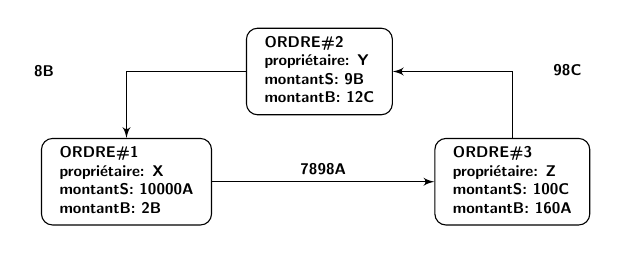
\begin{tikzpicture}[
    auto, 
    node distance=2cm,
    >=latex',
    font=\bfseries\footnotesize\sffamily,
    order/.style={
		scale=0.7,
		rectangle,
		rounded corners,
		draw=black, 
		text centered,
%		text width=5cm,
		minimum height=12mm,
		fill=white
	},
	label/.style={
		scale=0.7
	}
  ]
    % We start by placing the blocks

  \node [order] (order2) 
 {%
 \begin{tabular}{l}
  \textbf{ORDRE\#2}\\
  \textbf{propriétaire: Y}\\
  \textbf{montantS: 9B}\\
  \textbf{montantB: 12C}
 \end{tabular}
 };
 
  \node [order, below of=order2, xshift=-3.5cm] (order1) 
 {%
 \begin{tabular}{l}
  \textbf{ORDRE\#1}\\
  \textbf{propriétaire: X}\\
  \textbf{montantS: 10000A}\\
  \textbf{montantB: 2B}
 \end{tabular}
 };
 
 
  \node [order, below of=order2, xshift=3.5cm] (order3) 
 {%
 \begin{tabular}{l}
  \textbf{ORDRE\#3}\\
  \textbf{propriétaire: Z}\\
  \textbf{montantS: 100C}\\
  \textbf{montantB: 160A}
 \end{tabular}
 };
 
 \draw [draw,->] (order1) -- node [label] {\textbf{7898A}} (order3);
 \draw [draw,->] (order2) -| node [label, xshift=-1.8cm] {\textbf{8B}} (order1);
 \draw [draw,->] (order3) |- node [label, xshift=1cm, yshift=0.24cm] {\textbf{98C}} (order2);

\end{tikzpicture}

\caption{Un anneau d'ordres à 3 ordres}
\label{fig:ring}
\end{figurehere}
\end{center}


La figure ci-dessus montre un anneau d'ordres de 3 ordres. Chaque ordre de vente de jetons (\verb|jetonS|) est le jeton d'un autre ordre d'achat (\verb|jetonB|). Il crée une boucle qui permet à chaque ordre d'échanger les jetons souhaités sans avoir besoin d'un ordre opposé pour sa paire. Les paires d'ordres d’échanges traditionnelles peuvent, bien sûr, être exécutées dans ce qui est essentiellement un cas particulier d'un groupe d'ordres.

\begin{definition}[Anneau d'ordres] Soient $C_{0}$, $C_{1}$, $\cdots$, $C_{n-1}$,  $n$ jetons différents, et $O_{0\rightarrow 1}$, $\cdots$, $O_{i\rightarrow i\oplus 1}$, $\cdots$, $O_{n-1 \rightarrow 0}$ sont $n$ ordres. Ces ordres peuvent former un anneau d'ordre pour les échanges :

$$O_{0\rightarrow 1} \rightarrow \cdots \rightarrow O_{i\rightarrow i\oplus 1} \rightarrow \cdots \rightarrow O_{n-1\rightarrow 0} \text{, }$$
où $n$ est la longueur de l'anneau d'ordres, et $i\oplus 1 \equiv i+1 \mod n$.
\end{definition}

Un anneau d'ordres est valide lorsque toutes les transactions qui le compose peuvent être exécutées à un taux de change égal ou supérieur au taux initial spécifié implicitement par l'utilisateur. Pour vérifier la validité de l'anneau d’ordres, les contrats intelligent du protocol Loopring doivent recevoir des anneaux d’ordres de la part des mineurs d'anneau lorsque le produit des taux de change originaux de toutes les commandes est égal ou supérieur à 1.

Supposons qu'Alice et Bob veulent échanger leurs jetons \verb|A| et \verb|B|. Alice a  15 jetons \verb|A|et elle en veut 4 jetons \verb|B| en échange ; Bob a 10 jetons \verb|B| et il en veut 30 jetons \verb|A| en échange.

Qui achète et qui vend ? Cela dépend uniquement de l'actif que nous choisissons pour fixer les cotations de prix. Si le jeton \verb|A| est la référence, Alice achète le jeton \verb|B| pour le prix de ${15 \over 4 }= 3.75$ \verb|A|, tandis que Bob vend 10 jetons \verb|B| pour le prix de ${30 \over 10} = 3.00$ \verb|A|. Dans le cas où l’on choisit le jeton \verb|B| comme référence, nous disons qu'Alice vend 15 jeton \verb|A| pour le prix de ${4\over 15}=0.26666667$ \verb|B| et Bob achète 10 jetons \verb|A| pour le prix de ${10 \over 30}=0.3333333334$ \verb|B|. Par conséquent, dire qui est l'acheteur ou le vendeur est un choix arbitraire.

Dans la première situation, Alice est prête à payer un prix plus élevé ($3,75$\verb|A|) que le prix auquel Bob vend ses jetons (3$.00$\verb|A|), alors que dans la seconde situation Bob est prêt à payer un prix plus élevé ($0,33333334$\verb|B|) que le prix auquel Alice vend ses jetons ($0,2666666667$\verb|B|). Il est clair qu'une transaction est possible lorsque l'acheteur est prêt à payer un prix égal ou supérieur au prix du vendeur.

\begin{equation}
{{15\over 4} \over {30\over 10}} = {{10\over 30} \over {4\over 15}}={15 \over 4} \cdot {10 \over 30} = 1.25 > 1
\end{equation}

Ainsi, pour qu'un ensemble d'ordres $n$ puisse être rempli, totalement ou en partie, il faut savoir si le produit de chacun des taux de change comme les ordres d'achat se traduit par un nombre supérieur ou égal à 1. Si c'est le cas, tous les ordres $n$ peuvent être partiellement ou totalement exécutés \cite{supersymmetry}.

Si nous introduisons une troisième partie prenante, Charlie, de sorte qu'Alice veut donner $x_1$ jetons \verb|A| et recevoir $y_1$ jetons \verb|B|, Bob veut donner $x_2$ jetons \verb|B| et recevoir $y_2$ jetons \verb|C|, et Charlie veut donner $x_3$ jetons \verb|C| et recevoir $y_3$ jetons \verb|A|. Les jetons nécessaires sont présents, et le commerce est possible si :

\begin{equation}
{{x_1 \cdot x_2 \cdot x_3 \over y_1 \cdot y_2 \cdot y_3} \geq 1}
\end{equation}


Voir section \ref{anatomy} pour avoir plus de détails concernant les ordres de Loopring.



\section{Participants à l'écosystème\label{sec:ecosystem}}
Les participants à l'écosystème suivants fournissent conjointement toutes les fonctionnalités qu'un échange centralisé a à offrir. 

\begin{itemize}

\item \textbf{Portefeuilles} : Un service ou une interface pour les portefeuilles courant qui permet aux utilisateurs d'accéder à leurs jetons et d'envoyer des commandes au réseau Loopring. Les portefeuilles seront incités à produire des ordres en partageant les récompenses avec les mineurs (voir la section \ref{sec:token}). Ayant la conviction que l'avenir du trading n’aura lieu que grâce à la sécurité des portefeuilles des utilisateurs individuels, il est primordial de connecter les pools de liquidité par le biais de notre protocole.

\item \textbf{Chaîne de blocs de partage de liquidité/ maille de relais } : Un réseau de mailles de relais pour les ordres \& le partage de liquidité. Lorsque les nœuds exécutent le logiciel de relais Loopring, ils sont en mesure de rejoindre un réseau existant et de partager des liquidités avec d'autres relais par le biais d'un consortium de chaîne de blocs. Le consortium de chaîne de blocs que nous construisons en tant que première implémentation a un partage d'ordres en temps quasi réel (1-2 secondes par blocs), et réduit l'ancien historique pour permettre un téléchargement plus rapide pour les  nouveaux nœuds. Notamment, les relais n'ont pas besoin de se joindre à ce consortium ; ils peuvent agir seuls et ne pas partager la liquidité avec d'autres, ou, ils peuvent démarrer et gérer leur propre réseau de partage de liquidité.

\item \textbf{Relais/Mineurs d'anneaux} : Les relais sont des nœuds qui reçoivent des ordres des portefeuilles ou du maillage de relais, tiennent à jour les carnets d'ordres publics et l'historique des transactions, et éventuellement diffusent des ordres à d'autres relais (par l'intermédiaire de n’importe quel moyen hors chaîne) et/ou des nœuds de maillage de relais. Le minage en anneau est une caractéristique - et non une exigence - des relais. Il demande des capacités de calculs importantes et se fait complètement hors chaîne. Nous appelons relais, avec la fonction de minage d’ anneau activée, \enquote{les mineurs d’anneaux}, qui produisent des anneaux d'ordres en assemblant des ordres disparates. Les relais sont libres de choisir (1) comment ils communiquent entre eux, (2) comment ils construisent leurs carnets de commandes, et (3) comment ils exploitent les anneaux d'ordres (algorithmes de minage).

\item \textbf{Les contrats intelligents du Protocole Loopring(LPSC)} : Un ensemble de contrats intelligents publics et gratuits qui vérifie les anneaux d’ordres reçus des mineurs, règle et transfère sans confiance les jetons au nom des utilisateurs, incite les mineurs et les portefeuilles avec des récompenses, et émet des événements. Les relais/navigateurs d’ordres surveillent  ces événements pour tenir à jour leurs carnets de commandes et l'historique des transactions. Voir l'annexe \ref{app:protocol_ethereum} pour plus de détails.

\item \textbf{Services de création de jetons d'actifs (ATS)}: Un pont entre les actifs qui ne peuvent pas être négociés directement sur Loopring. Il s'agit de services centralisés gérés par des entreprises ou des organisations dignes de confiance. Les utilisateurs déposent des actifs (réels, fiat ou jetons d'autres chaînes) et obtiennent des jetons émis, qui peuvent être rachetés pour le dépôt à l'avenir. Loopring n'est pas un protocole d'échange inter-chaînes (jusqu'à ce qu'une solution appropriée existe), mais ATS permet de négocier des jetons ERC20 \cite{ERC20} avec des actifs physiques ainsi que des actifs sur d'autres chaînes de blocs.

\end{itemize}


\section{Processus d'échange\label{sec:process}}



\begin{enumerate} 


\item \textbf{Autorisation du protocole} : Dans la figure \ref{fig:process}, l'utilisateur \verb|Y| qui veut échanger des jetons autorise le LPSC à gérer le \verb|montantS|de jetons \verb|B| que l'utilisateur veut vendre. Cela ne bloque pas les jetons de l'utilisateur, qui reste libre de les déplacer pendant le traitement de la commande.

\item \textbf{Création d’ordres} : Le taux actuel et le carnet de commandes pour les jetons \verb|B| vs les jetons \verb|C|, sont fournis par des relais ou d'autres agents connectés au réseau, tels que les navigateurs de carnet de commandes. L'utilisateur \verb|Y| passe un ordre (ordre à cours limité) en spécifiant le\verb|montantS| et le \verb|montantB| et d'autres paramètres par le biais de n'importe quelle interface de portefeuille intégrée. Un montant de LRx peut être ajouté à la commande en tant que récompense pour les mineurs d'anneau ; des récompenses de LRx plus élevés signifient une meilleure chance d'être traités rapidement par les mineurs d'anneau. Le hash de la commande est signé avec la clé privée de l'utilisateur \verb|Y|.



\begin{center}
\begin{figurehere}
\centering
\tikzstyle{block} = [draw, fill=blue!20, rectangle, 
    minimum height=3em, minimum width=6em]
\tikzstyle{sum} = [draw, fill=blue!20, circle, node distance=1cm]
\tikzstyle{input} = [coordinate]
\tikzstyle{output} = [coordinate]
\tikzstyle{pinstyle} = [pin edge={to-,thin,black}]

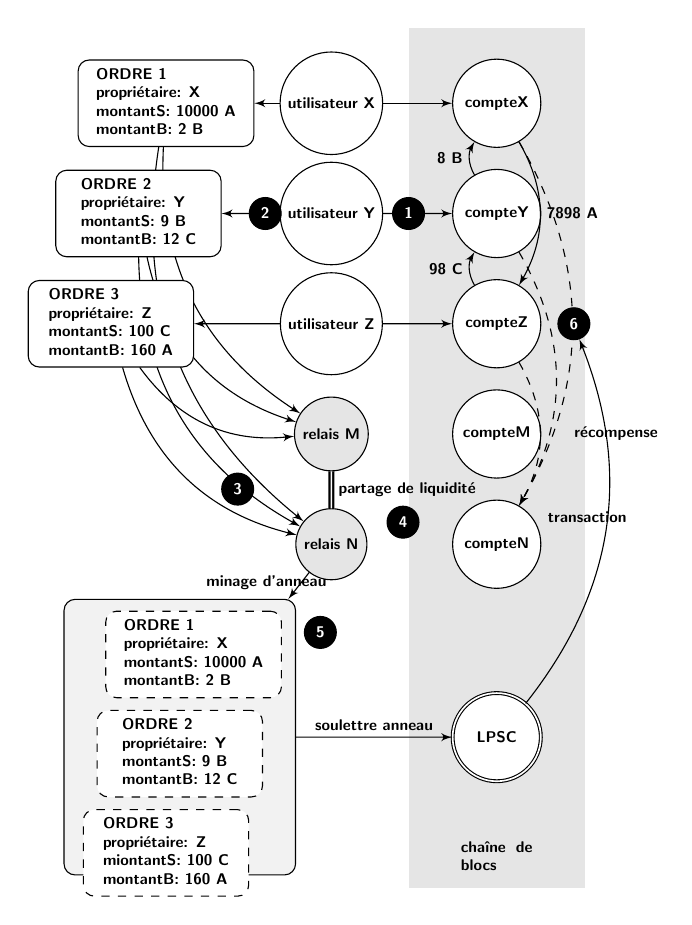
\begin{tikzpicture}[
    auto, 
    scale=0.7,
    node distance=2cm,
    >=latex',
    font=\bfseries\footnotesize\sffamily,
    order/.style={
		rectangle,
		scale=0.7,
		rounded corners,
		draw=black, 
		text centered,
%		text width=5cm,
		minimum height=12mm,
		minimum width=30mm,
		fill=white
	},
	role/.style={
		circle,
		scale=0.7,
		draw=black, 
		text centered,
%		text width=5cm,
		minimum height=12mm,
		minimum width=12mm,
		fill=white
	},
	steps/.style={
		circle,
		scale=0.7,
		draw=black, 
		text centered,
%		text width=5cm,
%		minimum height=12mm,
%		minimum width=12mm,
		fill=black,
		text=white
	},
	account/.style={
		circle,
		scale=0.7,
		draw=black, 
		text centered,
%		text width=5cm,
		minimum height=16mm,
		minimum width=16mm,
		fill=white
	},
	label/.style={
	  scale=0.7
    }
  ]

 
 \node [role] (user1)  {utilisateur X};
 \node [role, below of=user1] (user2)  {utilisateur Y};
 \node [role, below of=user2] (user3)  {utilisateur Z};
 \node [role, below of=user3, fill=gray!20] (relay1)  {relais M};
 \node [role, below of=relay1, fill=gray!20] (relay2)  {relais N};

 
 \node [order, left of=user1, xshift=-1cm] (order1) 
 {%
 \begin{tabular}{l}
  \textbf{ORDRE 1}\\
  \textbf{propriétaire: X}\\
  \textbf{montantS: 10000 A}\\
  \textbf{montantB: 2 B}
 \end{tabular}
 };
 
 \draw [draw, ->]  (user1) -- (order1) [label]{};
 \draw [bend right,->] (order1) to node [auto, scale=0.7] {} (relay1);
 \draw [bend right,->] (order1) to node [auto, scale=0.7] {} (relay2);
% \draw [draw, ->]  (order1) |- (relay1) [label]{};
% \draw [draw, ->]  (order1) |- (relay2) [label]{};
 
 \node [order,left of=user2, xshift=-1.5cm] (order2) 
 {%
 \begin{tabular}{l}
  \textbf{ORDRE 2}\\
  \textbf{propriétaire: Y}\\
  \textbf{montantS: 9  B}\\
  \textbf{montantB: 12 C}
 \end{tabular}
 };
 \draw [draw, ->]  (user2) -- (order2) [label]{};
 \draw [bend right,->] (order2) to node [auto, scale=0.7] {} (relay1);
 \draw [bend right,->] (order2) to node [auto, scale=0.7] {} (relay2);
% \draw [draw, ->]  (order2) |- (relay1) [label]{};
% \draw [draw, ->]  (order2) |- (relay2) [label]{};
% 
\node [order, left of=user3, xshift=-2cm] (order3) 
 {%
 \begin{tabular}{l}
  \textbf{ORDRE 3}\\
  \textbf{propriétaire: Z}\\
  \textbf{montantS: 100 C}\\
  \textbf{montantB: 160 A}
 \end{tabular}
 };
 \draw [draw, ->]  (user3) -- (order3) [label]{};
 \draw [bend right,->] (order3) to node [auto, scale=0.7] {} (relay1);
 \draw [bend right,->] (order3) to node [auto, scale=0.7] {} (relay2);
% \draw [draw, ->]  (order3) |- (relay1) [label]{};
% \draw [draw, ->]  (order3) |- (relay2) [label]{};
 
% // The Ring
\node [order, 
yshift=-1.5cm,
xshift=-2.75cm,
below of=relay2,
fill=gray!10,
minimum width=4.2cm,
minimum height=5cm] (ring) {};


\node [order, dashed, below of=relay2,yshift=-0.0cm,xshift=-2.5cm] (order11) 
 {%
 \begin{tabular}{l}
  \textbf{ORDRE 1}\\
  \textbf{propriétaire: X}\\
  \textbf{montantS: 10000 A}\\
  \textbf{montantB: 2 B}
 \end{tabular}
 };
 \node [order, dashed,below of=order11,xshift=-0.25cm,yshift=0.2cm] (order21) 
 {%
 \begin{tabular}{l}
  \textbf{ORDRE 2}\\
  \textbf{propriétaire: Y}\\
  \textbf{montantS: 9  B}\\
  \textbf{montantB: 12 C}
 \end{tabular}
 };
\node [order, dashed,below of=order21,xshift=-0.25cm,yshift=0.2cm] (order31) 
 {%
 \begin{tabular}{l}
  \textbf{ORDRE 3}\\
  \textbf{propriétaire: Z}\\
  \textbf{miontantS: 100 C}\\
  \textbf{montantB: 160 A}
 \end{tabular}
 };
 
 % // The blockchain
\node [
rectangle,
fill=gray!20, 
right of=user1,
yshift=-4.5cm,
xshift=0.1cm,
scale=0.7,
minimum width=3.2cm,
minimum height=15.6cm] (blockchain) {\parbox[b][15cm]{1.3cm}{chaîne de blocs}};
% blockchain accounts
  \node [account, right of=user1, xshift=1cm] (account1)  {compteX};
  \node [account, right of=user2, xshift=1cm] (account2)  {compteY};
  \node [account, right of=user3, xshift=1cm] (account3)  {compteZ};
  \node [account, right of=relay1, xshift=1cm] (account4)  {compteM};
  \node [account, right of=relay2, xshift=1cm] (account5)  {compteN};
  \node [account, double, below of=account5, yshift=-1.5cm] (psc)  {LPSC};
  
 \draw [draw, ->]  (user1) -- (account1) [label]{};
 \draw [draw, ->]  (user2) -- (account2) [label]{};
 \draw [draw, ->]  (user3) -- (account3) [label]{};
% \draw [draw, ->]  (relay1) -- (account4) [label]{};
% \draw [draw, ->]  (relay2) -- (account5) [label]{};
 \draw [draw, double, thick]  (relay1) to node [auto, scale=0.7] {partage de liquidité}  (relay2) [label]{};
% \draw [draw, ->]  (relay1) -- (ring) [label]{};
 \draw [draw, ->]  (relay2) to node [auto, scale=0.7, xshift=-1.8cm, yshift=0.3cm] {minage d'anneau}  (ring) [label]{};
 \draw [draw, ->]  (ring) to node [auto, scale=0.7] {soulettre anneau} (psc) [label]{};
 
 \draw [bend left,->] (account1) to node [auto, scale=0.7] {\textbf{7898 A}} (account3);
 \draw [bend left,->] (account2) to node [auto, scale=0.7] {\textbf{8 B}} (account1);
 \draw [bend left,->] (account3) to node [auto, scale=0.7] {\textbf{98 C}} (account2);
 
 \draw [bend left,->, dashed] (account1) to node [auto, scale=0.7] {} (account5);
 \draw [bend left,->, dashed] (account2) to node [auto, scale=0.7] {} (account5);
 \draw [bend left,->, dashed] (account3) to node [auto, scale=0.7, xshift=.5cm] {\textbf{récompense}} (account5);
  
  
% \draw [draw,->] (order1) -- node [label] {\textbf{7898 A}} (order3);
% \draw [draw,->] (order2) -| node [label, xshift=-1.8cm] {\textbf{8 B}} (order1);
% \draw [draw,->] (order3) |- node [label, xshift=1cm, yshift=0.24cm] {\textbf{98 C}} (order2);

\node [steps, right of=user2, xshift=-0.6cm] () {1};
\node [steps, left of=user2, xshift=0.8cm] () {2};
\node [steps, left of=relay2, xshift=0.3cm, yshift=1cm] () {3};
\node [steps, left of=relay1, xshift=3.3cm, yshift=-1.6cm] () {4};
\node [steps, below of=relay2, xshift=-0.2cm, yshift=0.4cm] () {5};
\node [steps, right of=account3, xshift=-0.6cm] (step5) {6};

 \draw [bend right, ->]  (psc) to node [auto, scale=0.7, xshift=0.5cm] {transaction} (step5) [label]{};
 
\end{tikzpicture}

\caption{Processus d'échange Loopring}
\label{fig:process}
\end{figurehere}
\end{center}

\item \textbf{Diffusion d’ordre} : Le portefeuille envoie la commande et sa signature à un ou plusieurs relais. Les relais mettent à jour leur carnet d'ordre public. Le protocole n'exige pas que les carnets de commandes soient construits d'une certaine façon, comme le principe du premier arrivé, premier servi. Au lieu de cela, les relais ont le pouvoir de prendre leurs propres décisions de conception en construisant leurs carnets de commandes.

\item \textbf{Partage de Liquidité} : Les relais diffusent l'ordre à d'autres relais par n'importe quel moyen de communication. Ici encore, il y a une certaine souplesse quant à la façon dont les nœuds interagissent. Pour faciliter un certain niveau de connectivité du réseau, il y a un relais de partage de liquidité intégré utilisant un consortium de chaîne de blocs. Comme mentionné dans la section précédente, ce maillage de relais est optimisé pour la vitesse et la globalité.


\item \textbf{Minage en anneaux (appariement des ordres)} : Les mineurs d’anneaux  essaient de satisfaire l’ordre entièrement ou partiellement au taux de change donné ,ou mieux, en l'appariant avec de multiples autres ordres. Le minage en anneau est la principale raison pour laquelle le protocole est capable de fournir une grande liquidité sur n'importe quelle paire. Si le taux d'exécution est meilleur que ce que l'utilisateur Y a spécifié, la marge est partagée entre tous les ordres dans l’anneau d’ordres. En guise de récompense, le mineur choisit entre réclamer une partie de la marge (partage de marge, et rendre le LRx à l'utilisateur), ou simplement garder les récompense de LRx.

\item \textbf{Vérification \& Transaction} : L'anneau d'ordre est reçu par le LPSC. Il effectue de multiples vérifications pour vérifier les données fournies par les mineurs d’anneau et détermine si l'anneau d’ordres peut être réglé entièrement ou partiellement (en fonction du taux d’accomplissement de l'anneau d’ordres et des jetons dans le portefeuille de l'utilisateur). Si tous les contrôles sont réussis, le contrat transfère "atomiquement" les jetons aux utilisateurs et paie en même temps le mineur d’anneau et les frais de portefeuille. Si le solde de l'utilisateur \verb|Y| tel que déterminé par le LPSC est insuffisant, il sera considéré comme réduit : un ordre réduit sera automatiquement ramené à sa taille originale si suffisamment de fonds sont déposés à son adresse, contrairement à une annulation, qui est une opération manuelle à sens unique et ne peut pas être annulée.

\end{enumerate}





%
%\end{multicols}
%
%\begin{center}
%\begin{figurehere}
%\includegraphics[height=8cm]{images/en_protocol.png}
%\caption{Loopring Trading Process}
%\label{fig: Loopringrotocol}
%\end{figurehere}
%\end{center}
%
%\begin{multicols}{2}

\section{Flexibilité opérationnelle\label{sec:business_model}}
Il est important de noter que le standard ouvert de Loopring permet aux participants une grande flexibilité dans la façon dont ils opèrent. Les acteurs sont libres de mettre en œuvre de nouveaux modèles d'affaires et de fournir de la valeur aux utilisateurs, en percevant des honoraires LRx sur le volume ou d'autres mesures dans le processus (s'ils le souhaitent). L'écosystème est modulaire et vise à soutenir la participation à partir d'une multitude d'applications.


\subsection{Carnet de commande\label{sec:order_book}}
Les relais peuvent concevoir leurs carnets de commandes de différentes manières pour afficher et faire correspondre les ordres des utilisateurs. Une première mise en œuvre de notre propre carnet d'ordres suit un modèle OTC, où les ordres à cours limité sont positionnés sur la seule base du prix. En d'autres termes, l'horodatage des commandes n'a aucune incidence sur le carnet de commandes. Cependant, un relais est libre de concevoir son carnet d'ordres de manière à imiter le moteur d'appariement d'une place d’échanges centralisée typique, où les ordres sont classés par prix, tout en respectant les horodatages. Si un relais était enclin à offrir ce type de carnet de commandes, ils peuvent posséder ou s'intégrer avec un portefeuille, et faire envoyer ces commandes de portefeuille exclusivement au relais unique, qui serait alors en mesure d'apparier les ordres en fonction du temps. Une telle configuration est possible.

Alors que d'autres protocoles DEX exigent parfois des relais d'avoir des ressources - des soldes de jetons initiaux pour passer des ordres de preneur - les relais Loopring n'ont besoin que de trouver des ordres compatibles pour effectuer une transaction, et peuvent le faire sans jetons initiaux.

\subsection{Partage de liquidité\label{sec:liquidity_sharing}}
Les relais sont libres de concevoir comment ils partagent la liquidité (ordres) les uns avec les autres. Notre consortium de chaîne de blocs n'est qu'une solution pour y parvenir, et l'écosystème est libre de se mettre en réseau et de communiquer comme ils le souhaitent. En plus de se joindre à un consortium, ils peuvent construire et gérer leur propre chaîne de blocs, en créant des règles/incitations comme ils l'entendent. Les relais peuvent aussi fonctionner seuls, comme on peut le voir dans la mise en place d'un portefeuille sensible au temps. Bien sûr, il y a des avantages évidents à communiquer avec d'autres relais dans la recherche d'effets de réseau, cependant, différents modèles d'affaires pourraient mériter des conceptions particulières de partage et des frais partagés de plusieurs façons.

\section{Spécification du protocole\label{sec:protocol}}

\subsection{Anatomie d'un ordre\label{anatomy}}
Une commande est un ensemble de données qui décrit l'intention de donner un ordre de l'utilisateur. Un ordre Loopring est défini à l'aide du modèle d'ordre unidirectionnel, ou UDOM, comme suit :

\begin{verbatim}
  message Order {
    address protocol;
    address owner;
    address tokenS;
    address tokenB;
    uint256 amountS;
    uint256 amountB;
    unit256 lrcFee
    unit256 validSince; // Seconds since epoch
    unit256 validUntil; // Seconds since epoch
    uint8   marginSplitPercentage;  // [1-100]
    bool    buyNoMoreThanAmountB;
    uint256 walletId;
    // Dual-Authoring address
    address authAddr;
   	// v, r, s are parts of the signature
    uint8   v;       
    bytes32 r;
    bytes32 s;
    // Dual-Authoring private-key,
    // not used for calculating order's hash,
    // thus it is NOT signed.
    string  authKey;          
  }
\end{verbatim}


Pour assurer l'origine de l’ordre, il est signée avec le hachage de ses paramètres, à l'exclusion de \verb|authAddr|, avec la clé privée de l'utilisateur. Le paramètre \verb|authAddr| est utilisé pour signer les anneaux d'ordre dont cet ordre fait partie, ce qui empêche le front-running. Veuillez vous référer à la section \ref{sec:dual_authoring} pour plus de détails. La signature est représentée par les champs \verb|v|, \verb|r|, et \verb|s|, et est envoyée avec les paramètres de l'ordre sur le réseau. Ceci garantit que la commande reste immuable pendant toute sa durée de vie. Même si l'ordre ne change jamais, le protocole peut toujours calculer son état actuel en fonction du solde de son adresse et d'autres variables.



L'UDOM n'inclut pas un prix (qui doit être un nombre à virgule flottante par nature), mais utilise plutôt le terme \verb|rate| ou $r$, qui est exprimé en \verb|montantS|/\verb|montantS|/\verb|montantB|. Le taux n'est pas un nombre à virgule flottante mais une expression qui ne sera évaluée qu'avec d'autres entiers non signés sur demande, afin de conserver tous les résultats intermédiaires comme entiers non signés et d'augmenter la précision du calcul.

\subsubsection{Montants d'achat}

Quand un mineur d’anneau exécute un ordre, il est possible qu'un meilleur taux soit alors exécutable, permettant aux utilisateurs d'obtenir plus de \verb|jetonB| que le \verb|montantB| qu'ils ont spécifié. Cependant, si \verb|buyNoMoreThanAmountB| est réglé sur \verb|True|, le protocole garantit que les utilisateurs ne reçoivent pas plus que \verb|montantB| de \verb|jetonB| de \verb|jetonB|. Ainsi, le paramètre UDOM \verb|buyNoMoreThantokenB| détermine quand une commande est considérée comme complètement remplie. \verb|buyNoMoreThantokenB| applique un plafond sur les montants \verb|montantS| ou \verb|montantB|, et permet aux utilisateurs d'exprimer des intentions plus fines que les ordres d'achat/de vente traditionnels.

Par exemple : avec \verb|montantS| = 10 et \verb|montantB| = 2, le taux $r$ = 10/2 = 5. Ainsi, l'utilisateur est prêt à vendre 5 \verb|jetonS| pour chaque \verb|jetonB|. Le mineur d’anneaux travaille et trouve pour l'utilisateur un taux de 4, permettant à l'utilisateur de recevoir 2,5 \verb|jetonB| au lieu de 2. Cependant, si l'utilisateur ne veut que 2 \verb|jetonB| et met le drapeau \verb|buyNoMoreThanAmountB| sur \verb|True|, le LPSC effectue la transaction à un taux de 4 et l'utilisateur vend 4 \verb|jetonS| pour chaque \verb|jetonB|, sauvegardant ainsi 2 \verb|jetonS|. Gardez à l'esprit que ceci ne tient pas compte des frais de minage (voir section \ref{sec:fee_model}).
En effet, si l'on utilise :


\begin{verbatim}
	      Order(amountS,tokenS,
	            amountB,tokenB,
	            buyNoMoreThantokenB)
\end{verbatim}

pour représenter un ordre sous une forme simplifiée, alors pour les marchés ETH/USD sur une place d’échanges traditionnelle, le modèle traditionnel d'achat-vente peut exprimer le 1er et le 3ème ordre ci-dessous, mais pas les deux autres :

\begin{enumerate}
	\item Vendre 10 ETH au prix de 300 USD/ETH. Cet ordre peut être exprimé de la façon suivante : \verb|Order(10, ETH, 3000, USD, False)|.
	\item Vendre ETH au prix de 300 USD/ETH pour obtenir 3000 USD. Cet ordre peut être exprimé de la façon suivante: \verb|Order(10, ETH, 3000, USD, True)|.
	\item Acheter 10 ETH au prix de 300 USD/ETH, Cet ordre peut être exprimé de la façon suivante: \verb|Order(3000, USD, 10, ETH, True)|.
	\item Dépenser 3000 USD pour acheter autant d'ETH que possible au prix de 300 USD/ETH, Cet ordre peut être exprimé de la façon suivante: \verb|Order(3000, USD, 10, ETH, False)|.
\end{enumerate}



\subsection{Vérification de l'anneau\label{sec:ring_verification}}

Les contrats intelligents Loopring n'effectuent pas de calculs de taux de change ou de montant, mais doivent recevoir et vérifier ce que les mineurs d’anneaux fournissent pour ces valeurs. Ces calculs sont effectués par les mineurs d’anneau pour deux raisons principales : (1) le langage de programmation pour les contrats intelligents, comme solidity\cite{dannen2017introducing} sur Ethereum, ne supporte pas les calculs avec  virgule flottante, en particulier $pow(x, 1/n)$ (calcul de la n-ème racine d'un nombre à virgule flottante), et (2) il est souhaitable que le calcul soit effectué hors chaîne pour réduire l’impact en termes de poids de calcul et de coût.


\subsubsection{Vérification des sous-anneaux\label{sec:sub_ring_check}}
Cette étape empêche les arbitragistes de capter injustement toute la marge dans un anneau ‘ordres en mettant en œuvre de nouveaux ordres au sein d’un anneau. Effectivement, une fois qu'un anneau d'ordre valide est trouvé par un mineur d’anneaux, il pourrait être tentant d'ajouter d'autres ordres à cet anneau pour absorber complètement la marge des utilisateurs (rabais de taux). Comme illustré par la figure \ref{fig:subring} ci-dessous, un calcul méticuleux de $x1$, $y1$, $y1$, $x2$ et $y2$ fera en sorte que le produit de toutes les commandes soit exactement 1, donc il n'y aura pas de réduction de taux.

\begin{center}
\begin{figurehere}
\centering
\tikzstyle{block} = [draw, fill=blue!20, rectangle, 
    minimum height=3em, minimum width=6em]
\tikzstyle{sum} = [draw, fill=blue!20, circle, node distance=1cm]
\tikzstyle{input} = [coordinate]
\tikzstyle{output} = [coordinate]
\tikzstyle{pinstyle} = [pin edge={to-,thin,black}]

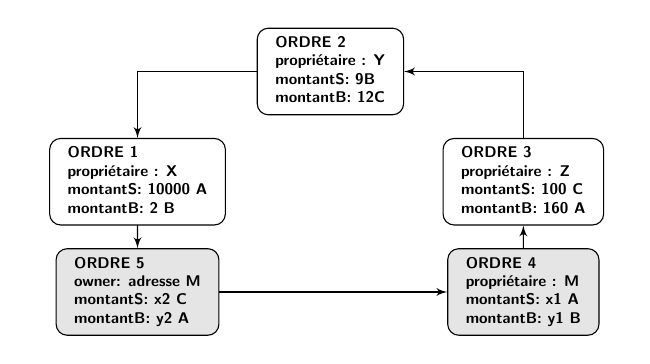
\begin{tikzpicture}[
    auto, 
    node distance=2cm,
    >=latex',
    font=\bfseries\footnotesize\sffamily,
    order/.style={
		scale=0.7,
		rectangle,
		rounded corners,
		draw=black, 
		text centered,
%		text width=5cm,
		minimum height=12mm,
		fill=white
	},
	label/.style={
		scale=0.7
	}
  ]
    % We start by placing the blocks

  \node [order] (order2) 
 {%
 \begin{tabular}{l}
  \textbf{ORDRE 2}\\
  \textbf{propriétaire : Y}\\
  \textbf{montantS: 9B}\\
  \textbf{montantB: 12C}
 \end{tabular}
 };
 
  \node [order, below of=order2, xshift=-3.5cm] (order1) 
 {%
 \begin{tabular}{l}
  \textbf{ORDRE 1}\\
  \textbf{propriétaire : X}\\
  \textbf{montantS: 10000 A}\\
  \textbf{montantB: 2 B}
 \end{tabular}
 };
 
 
  \node [order, below of=order2, xshift=3.5cm] (order3) 
 {%
 \begin{tabular}{l}
  \textbf{ORDRE 3}\\
  \textbf{propriétaire : Z}\\
  \textbf{montantS: 100 C}\\
  \textbf{montantB: 160 A}
 \end{tabular}
 };
 
   \node [order, below of=order3, fill=gray!20] (order4) 
 {%
 \begin{tabular}{l}
  \textbf{ORDRE 4}\\
  \textbf{propriétaire : M}\\
  \textbf{montantS: x1 A}\\
  \textbf{montantB: y1 B}
 \end{tabular}
 };
 
 
  \node [order, below of=order1, fill=gray!20] (order5) 
 {%
 \begin{tabular}{l}
  \textbf{ORDRE 5}\\
  \textbf{owner: adresse M}\\
  \textbf{montantS: x2 C}\\
  \textbf{montantB: y2 A}
 \end{tabular}
 };
 
 \draw [draw,->] (order1) -- node [label, xshift=-2cm] {} (order5);
 \draw [draw,->] (order2) -| node [label, xshift=-1.6cm] {} (order1);
 \draw [draw,->] (order3) |- node [label, xshift=1cm] {} (order2);
 \draw [draw,->] (order4) -- node [label, xshift=1.8cm] {} (order3);
 \draw [draw,->] (order5) -- node [label, yshift=0.2cm] {} (order4);
  
\end{tikzpicture}

\caption{Un anneau d'ordres avec sous-anneau}
\label{fig:subring}
\end{figurehere}
\end{center}

Il s'agit d'un risque nul, d'une valeur ajoutée nulle pour le réseau et d'un comportement déloyal de la part du mineur d’anneau. Pour éviter cela, Loopring exige qu'une boucle valide ne puisse pas contenir de sous-anneaux. Pour vérifier cela, le LPSC s'assure qu'un jeton ne peut pas être à la fois en position d'achat ou de vente. Dans le diagramme ci-dessus, nous pouvons voir que le jeton \verb|A| est à la fois un jeton de vente et un jeton d'achat, ce qui serait refusé.


\subsubsection{
Vérification du taux de réalisation\label{sec:fill_rate_check}}


Les calculs du taux de change dans l'anneau d'ordrse sont effectués par les mineurs d'anneau pour les raisons indiquées ci-dessus. C'est le LPSC qui doit vérifier qu'ils sont corrects. Tout d'abord, il vérifie que le taux d'achat que le mineur d’anneaux peut exécuter pour chaque ordre est égal ou inférieur au taux d'achat initial fixé par l'utilisateur. Cela permet de s'assurer que l'utilisateur obtient au moins le taux de change qu'il a demandé ou mieux sur la transaction. Une fois que les taux de change sont confirmés, le LPSC s'assure que chaque ordre dans l'anneau d'ordres partage le même rabais de taux. Par exemple, si le taux d'escompte est $\gamma$, alors le prix de chaque commande sera :

$r_{0\rightarrow 1} \cdot (1-\gamma)$, $r_{1\rightarrow 2} \cdot (1-\gamma)$, $r_{2 \rightarrow 0} \cdot (1-\gamma)$, et satisfait : 
\begin{equation}
r_{0\rightarrow 1} \cdot (1-\gamma)\cdot r_{1\rightarrow 2} \cdot (1-\gamma) \cdot r_{2 \rightarrow 0} \cdot (1-\gamma) = 1
\end{equation}
d'où : 
\begin{equation}
\gamma = 1- \frac{1}{\sqrt[3]{r_{0\rightarrow 1} \cdot r_{1\rightarrow 2} \cdot r_{2\rightarrow 0}}}\text{.}
\end{equation}
Si la transaction dépasse $n$ ordres, le \texttt{rabais} est: 
\begin{equation}
\gamma = 1- \frac{1}{\sqrt[n]{\prod_{i=0}^{n-1} r^i}} \text{,}
\end{equation}

où $r^i$ est le taux de rotation des ordres du $i$-ème ordre. Évidemment, c’est seulement quand le taux d'escompte est $\gamma\ge 0$, que ces ordres peuvent être exécutés ; et le taux de change réel du $i$-ème ordre ($O^i$) est $\hat{r^i} = r^i \cdot (1-\gamma)$, $\hat{r^i}\le r^i$.


\subsubsection{Suivi des transactions \& Annulation}

Un utilisateur peut annuler partiellement ou totalement une commande en envoyant une transaction spéciale au LPSC, contenant les détails de la commande et les montants à annuler. Le LPSC prend cela en compte, stocke les montants à annuler et émet un événement \verb|OrderCancelled| au réseau. Le LPSC garde la trace des montants remplis et annulés en stockant leurs valeurs en utilisant le hachage de l'ordre comme identificateur. Ces données sont accessibles au public et les événements \verb|OrderCancelled| / \verb|OrderFilled| sont émis lorsqu'ils changent. Le suivi de ces valeurs est essentiel pour le LPSC pendant l'étape de règlement du cycle d'ordres.

Le LPSC prend également en charge l'annulation de tous les ordres pour toute paire d’échange avec l'événement \verb|OrdersCancelled| et l'annulation de tous les ordres pour une adresse avec l'événement \verb|AllOrdersCancelled|.


\subsubsection{Échelonnement des ordres\label{sec:order_scaling}}
Les ordres sont échelonnées en fonction de l'historique des montants exécutés et annulés et du solde courant des comptes des expéditeurs. Le processus recherche l'ordre avec le plus petit montant à remplir en fonction des caractéristiques ci-dessus et l'utilise comme référence pour l'échelonnement de toutes les transactions dans le cycle d'ordre.


Trouver l'ordre de la valeur la plus basse peut aider à déterminer le volume de remplissage pour chaque commande. Par exemple, si le $i$-ème ordre est l'ordre de valeur la plus basse, alors le nombre de jetons vendus de chaque ordre $\hat{s}$ et le nombre de jetons achetés $\hat{b}$ de chaque ordre peut être calculé comme suit :

\[
\begin{split}
&\hat{s}^{i}=\overline{s}_i\text{, } \hat{b}^{i}=\hat{s}^{i}/ \hat{r}^i\text{, }\text{;}\\
&\hat{s}^{i\oplus 1}=\hat{b}^i\text{, } \hat{b}^{i\oplus 1}=\hat{s}^{i\oplus 1}/ \hat{r}^{i\oplus 1}\text{;}\\
&\hat{s}^{i\oplus 2}=\hat{b}^{i\oplus 1}\text{, } \hat{b}^{i\oplus 2}=\hat{s}^{i\oplus 2}/ \hat{r}^{i\oplus 2}\text{;}\\
& ...
%\text{.}
\end{split}
\]
où $\overline{s}_i$ est le solde restant après l'exécution partielle des ordres.

Au cours de la mise en œuvre, nous pouvons en toute sécurité assumer n'importe quel ordre dans l'anneau d'ordres pour avoir la valeur la plus basse, puis itérer à travers l'anneau d'ordres au plus deux fois pour calculer le volume de remplissage de chaque ordre. 

Exemple : si la plus petite quantité à remplir par rapport à l'ordre d'origine est de 5\%, toutes les transactions de l'anneau d'ordres sont réduites de 5\%. Une fois les transactions terminées, l'ordre qui était considéré comme ayant le plus petit montant restant à remplir devrait être complètement rempli.

\subsection{Transaction en anneau\label{sec:settlement}}

Si l'anneau d'ordres remplit toutes les vérifications précédentes, l'anneau d'ordre peut être clôturé et des transactions peuvent être effectuées. Cela signifie que tous les ordres $n$ forment un anneau d'ordres fermé, connecté comme dans la figure 4 :

\begin{center}
\begin{figurehere}
\centering
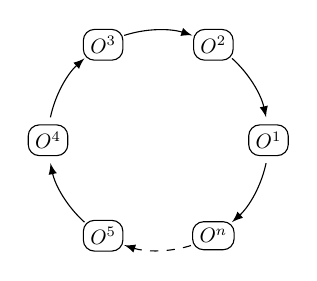
\begin{tikzpicture}[
circle/.style={
		scale=0.75,
		rounded corners,
		draw=black, 
		text centered,
		}
]

\def \n {6}
\def \m {4}
\def \radius {1.4cm}
\def \margin {12} % margin in angles, depends on the radius

\foreach \s in {1,...,\m}
{
  \node[draw, circle] at ({360/\n * (\s - 1)}:\radius) {$O^\s$};
  \draw[<-, >=latex] ({360/\n * (\s - 1)+\margin}:\radius) 
    arc ({360/\n * (\s - 1)+\margin}:{360/\n * (\s)-\margin}:\radius);
}

\node[draw, circle] at ({360/\n * 4}:\radius) {$O^5$};
  \draw[<-, dashed, >=latex] ({360/\n * 4+\margin}:\radius) 
    arc ({360/\n * 4+\margin}:{360/\n * (5)-\margin}:\radius);
    
\node[draw, circle] at ({360/\n * 5}:\radius) {$O^n$};
  \draw[<-, >=latex] ({360/\n * 5+\margin}:\radius) 
    arc ({360/\n * 5+\margin}:{360/\n * (6)-\margin}:\radius);


\end{tikzpicture}
\caption{Transaction en anneau}
\label{fig:settlement}
\end{figurehere}
\end{center}

Pour effectuer les transactions, le LPSC utilise le contrat intelligent \verb|TokenTransferDelegate|. L'introduction d'un tel représentant facilite la mise à jour du protocole du contrat intelligent puisque toutes les commandes doivent seulement autoriser ce représentant au lieu de versions différentes du protocole.

Pour chaque commande de l'anneau d'ordres, un paiement de \verb|JetonS| est effectué à la commande suivante ou précédente en fonction de l'exécution. Ensuite, les frais pour le mineur d’anneaux sont payés en fonction du modèle qu’il a choisit. Enfin, une fois que toutes les transactions sont effectuées, un événement \verb|RingMined| est émis.

\subsubsection{Événements émis\label{sec:events}}

Le protocole émet des événements qui permettent aux relais, aux navigateurs d'ordres et aux autres acteurs de recevoir les mises à jour du carnet de commandes aussi efficacement que possible. Les événements émis sont :

\begin{itemize}
	\item \textbf{OrderCancelled}: Un ordre particulier a été annulée.
	\item \textbf{OrdersCancelled}: Tous les ordres d'une paire d’échange à partir d'une adresse propre ont été annulés.
	\item \textbf{AllOrdersCancelled}: Tous les ordres de toutes les paires d’échange à partir d'une adresse propre ont été annulés.
	\item \textbf{RingMined}: Un anneau d'ordres a été établi avec succès. Cet événement contient les données relatives à chaque transfert de jeton de l'anneau intérieur.
\end{itemize}


\section{Jetons LRx\label{sec:token}}
LRx est notre façon générique de nommer les jetons.. LRC est le jeton Loopring sur Ethereum, LRQ sur Qtum, et LRN sur NEO, etc. D'autres types de LRx seront introduits à l'avenir à mesure que Loopring sera déployé sur d'autres chaînes de blocs publics.

\subsection{Modèle de frais\label{sec:fee_model}} 
Lorsqu'un utilisateur crée un ordre, il spécifie un montant de LRx à payer au mineur d’anneau en tant que frais, en conjonction avec un pourcentage de la marge (\verb|marginSplitPercentage|) réalisée sur la commande que le mineur d’anneau peut réclamer. C'est ce qu'on appelle le fractionnement de la marge. Le choix fait (frais ou partage de la marge) appartient  au mineur d’anneau.

Représentation du fractionnement de la marge :

\begin{center}
\begin{figurehere}
\centering
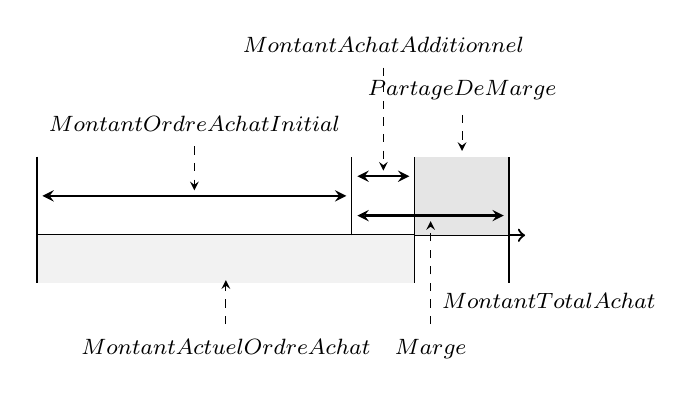
\begin{tikzpicture}[
scale=1,
font=\bfseries\footnotesize\sffamily,
classical/.style={thick,<->,shorten >=2pt,shorten <=2pt,>=stealth},
oneway/.style={->,dashed,shorten >=2pt,shorten <=2pt,>=stealth}
]
    % Draw axes
    \draw [->,thick] (0,1) node (yaxis) [above] {$$}
        |- (6.2,0) node (xaxis) [right] {$$};
        
    \draw
  	(4,0) coordinate (A)
  	(4,1) coordinate (A2)
  	(4.8,-0.6) coordinate (B)
  	(4.8,1) coordinate (B2)
  	(6,-0.6) coordinate (C)
  	(6,1) coordinate (C2);
  	
  	\fill [draw=none, fill=gray!20] 
    (4.8, 0) rectangle (6, 1);
    
  	\fill [draw=none, fill=gray!10] 
    (0, -0.6) rectangle (4.8, 0);

	\draw[thick] (0, -0.6) -- (0, 0.6) node[below]{$$};
  	\draw[thick, thin] (A) -- (A2) node[below]{$$};
  	\draw[thick, thin] (B) -- (B2) node[below]{$$};
  	\draw[thick] (C) node[below, xshift=0.5cm]{$Montant Total Achat$} -- (C2) ;
  	
  	\draw[classical] (0, 0.5) -> (4, 0.5) node[below]{$$};
  	\draw[classical] (4, 0.75) -> (4.8, 0.75) node[below]{$$};
%  	\draw[classical] (4.8, 0.5) -> (6, 0.5) node[below]{$$};
  	\draw[classical] (4, 0.25) -> (6, 0.25) node[below]{$$};

  	
  	\draw[oneway] (2, 1.2) node[above]{$Montant Ordre Achat Initial$} -- (2, 0.5);
  	\draw[oneway] (4.4, 2.2) node[above]{$Montant Achat Additionnel$} -- (4.4, 0.75);
  	\draw[oneway] (5.4, 1.6) node[above]{$Partage De Marge$} -- (5.4, 1);
  	\draw[oneway] (5, -1.2) node[below]{$Marge$} -- (5, 0.25);
  	\draw[oneway] (2.4, -1.2) node[below]{$Montant Actuel Ordre Achat$} -- (2.4, -0.5);



\end{tikzpicture}
\caption{Un partage de marge de 60\%}
\label{fig:marginsplit}
\end{figurehere}
\end{center}

Si la marge sur l'anneau d'ordres est trop petite, un mineur d’anneau  choisira les frais de LRx. Si, au contraire, la marge est suffisamment importante pour que le partage de la marge qui en résulte ait une valeur beaucoup plus élevée que les frais de LRx, le mineur choisira le partage de la marge. Il y a toutefois une autre condition : lorsque le mineur choisit le partage de la marge, il doit payer à l'utilisateur (créateur de l'ordre) une redevance, qui est égale au LRx que l'utilisateur aurait payé au mineur en tant que redevance. Cela augmente le seuil à partir duquel le mineur choisira le partage de la marge jusqu'à deux fois les frais LRx de l'ordre, ce qui augmente la propension au choix des frais LRx. Ceci permet aux mineurs d'anneau de recevoir un revenu constant sur les anneaux d'ordres à faible marge avec le compromis de recevoir moins de revenu sur les anneaux d'ordres à marge plus élevée. Notre modèle d'honoraires est basé sur le fait qu'au fur et à mesure que le marché va croître et arrive à maturité, il y aura moins d'anneaux d'ordres à marge élevée, ce qui nécessitera des frais fixes de LRx comme récompense.


Nous arrivons finalement au graphique suivant :

\begin{center}
\begin{figurehere}
\centering
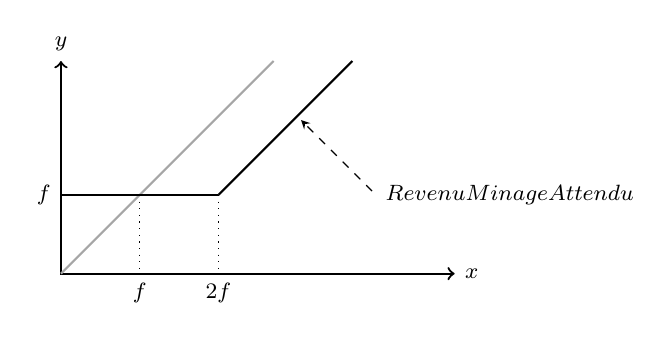
\begin{tikzpicture}[
font=\bfseries\footnotesize\sffamily,
oneway/.style={->,dashed,shorten >=2pt,shorten <=2pt,>=stealth},
scale=1]
    % Draw axes
    \draw [<->,thick] (0,2.7) node (yaxis) [above] {$y$}
        |- (5,0) node (xaxis) [right] {$x$};
        
    \draw
  	(1,1) coordinate (A)
  	(2,1) coordinate (B);
  	
  	
  	\draw[thick] (B) -- (3.7,2.7);
  	\draw[dotted] (B) -- (2,0) node[below] {$2f$};
  	\draw[dotted] (A) -- (1,0) node[below] {$f$};
  	\draw[thick,color=gray!70] (0,0) -- (2.7,2.7);
  	\draw[thick] (0,1) node[left] {$f$}--(B) node[     ]{$$};
 	\draw[oneway] (4,1) node[right]{$Revenu Minage Attendu$} -- (3, 2);


\end{tikzpicture}
\caption{Modèle de frais Loopring}
\label{fig:feemodel}
\end{figurehere}
\end{center}


où $f$ est la commission LRx, $x$ est le partage de la marge, $y$ est le revenu du minage. $y=max(f, x-f)$ comme indiqué par la ligne en trait plein ; si les frais de LRx pour l'ordre est $0$, l'équation est $y=max(0, x - 0)$ ce qui se simplifie à $y=x$ comme indiqué par la ligne grise.


Les conséquences sont :  
\begin{enumerate}
	\item Si le partage de la marge est de 0, les mineurs d’anneau choisiront le forfait LRx et seront toujours récompensés.
	\item Si les frais de LRx sont de 0, le résultat de la ligne grise et le revenu est basé sur un modèle linéaire général.
	\item Quand le revenu du partage de la marge est supérieur à 2x(LRx fee), les mineurs d’anneau choisissent le partage de la marge et paient LRx à l'utilisateur.

\end{enumerate}

Il convient de noter que si les frais de LRx ne sont pas nuls, quelle que soit l'option choisie par le mineur d’anneau, il y aura toujours un transfert de LRx entre le mineur d’anneau et l'expéditeur de l'ordre. Soit le mineur d’anneau gagne les frais de LRx, soit il rembourse les frais de LRx à l'expéditeur pour prendre le partage de la marge.

Les mineurs d'anneaux partageront un certain pourcentage des frais avec les portefeuilles. Lorsqu'un utilisateur passe un ordre via un portefeuille et qu'il est satisfait, le portefeuille est récompensé par une partie des frais ou du partage de la marge. Bien que cela soit modulaire et que des modèles d'affaires ou des implémentations uniques soient possibles, notre tendance est que les portefeuilles reçoivent environ 20\%-25\% des frais  gagnés. Les portefeuilles représentent une cible principale pour l'intégration du protocole Loopring car ils ont une base d'utilisateurs, mais peu ou pas de source de revenu.

\subsection{Gouvernance décentralisée}
À la base, le protocole Loopring est un protocole social en ce sens qu'il repose sur la coordination entre ses membres pour fonctionner efficacement vers un but. Cela n'est pas différent des protocoles crypto-économiques au sens large, et en effet, son utilité est largement protégée par les mêmes mécanismes de problèmes de coordination \cite{vitalikgovernance}, un équilibre "grim trigger" et une rationalité limitée. A cette fin, les jetons LRx ne sont pas seulement utilisés pour payer les frais, mais aussi pour harmoniser les incitations financières des différents participants au réseau. Un tel ajustement est nécessaire pour l'adoption à grande échelle de tout protocole, mais il est particulièrement important pour les protocoles d'échange, étant donné que le succès repose en grande partie sur l'amélioration de la liquidité dans un écosystème décentralisé robuste.

Les jetons LRx seront utilisés pour effectuer des mises à jour de protocole par le biais d'une gouvernance décentralisée. Les mises à jour  des contrats intelligents seront régies par les détenteurs de jetons afin d'assurer la continuité et la sécurité et d'atténuer les risques de liquidité siphonnée par une incompatibilité. Étant donné que les contrats intelligents ne peuvent pas être modifiés une fois déployés, il existe un risque que les dApps ou les utilisateurs finaux continuent d'interagir avec des versions obsolètes et s'excluent eux-mêmes des contrats mis à jour. L'évolutivité est cruciale pour le succès du protocole car il doit s'adapter aux demandes du marché et aux chaînes de blocs sous-jacentes. La gouvernance décentralisée par les parties prenantes de LRx permettra de mettre à jour les contrats intelligents sans perturber les dApps ou les utilisateurs finaux, ou en s'appuyant trop sur l'abstraction des contrats intelligents. Dans un premier temps, cela se fera par le biais d'un simple contrat intelligent multisignature, en vue de progresser vers un mécanisme de type DAO.

\section{Protections contre les fraudes et les attaques}

\subsection{Prévention du Front-running\label{sec:dual_authoring}}

Dans les places d’échanges décentralisés, le front-running se produit lorsque quelqu'un essaie de copier la solution d’échange d'un autre nœud et de la faire miner avant la transaction originale qui est dans le pool de transactions en attente (mempool). Ceci peut être réalisé en spécifiant des frais de transaction plus élevés (prix du gas). Le schéma principal du front-running dans Loopring (et tout protocole pour l'appariement des ordres) est le voleur-d’ordre : lorsqu'un front-runner vole un ou plusieurs ordres d'une transaction de règlement d'ordre en attente ; et, spécifique à Loopring : lorsqu'un front-runner vole l'ensemble de l'ordre d'une transaction en attente.


Lorsqu'une transaction submitRing n'est pas confirmée et se trouve toujours dans le pool de transactions en attente, n'importe qui peut facilement la repérer et remplacer \verb|minerAddress| par sa propre adresse (l'adresse \verb|filcherAddress|), alors ils peuvent re-signer la charge utile avec \verb|filcherAddress| pour remplacer la signature de l'anneau d’ordre.  Le fincher peut fixer un prix du gas plus élevé et soumettre une nouvelle transaction en espérant que les mineurs de bloc choisiront sa nouvelle transaction dans le bloc suivant au lieu de la transaction originale.

Les solutions précédentes à ce problème présentaient d'importants inconvénients : il fallait plus de transactions et donc plus de gaz pour les mineurs d’anneaux ; et il fallait au moins deux fois plus de blocs pour régler un anneau d'ordres.  Notre nouvelle solution, le Dual Authoring\cite{dualauthor}, implique le mécanisme de mise en place de deux niveaux d'autorisation pour les ordres - l'un pour le règlement et l'autre pour le minage en anneaux.

Processus de double création :

\begin{enumerate}

	\item Pour chaque commande, le logiciel de portefeuille génère une paire aléatoire clé publique/clé privée, et place la paire de clés dans l’extrait JSON de la commande. (Une alternative est d'utiliser l'adresse dérivée de la clé publique au lieu de la clé publique elle-même pour réduire le nombre d’octets nécessaires. Nous utilisons \verb|authAddr| pour représenter une telle adresse, et \verb|authKey| pour représenter la clé privée correspondante de \verb|authAddr|).

	\item Calculez le hachage de l'ordre avec tous les champs de l'ordre sauf \verb|r|, \verb|v|, \verb|s|, et \verb|authKey|), et signez le hachage en utilisant la clé privée du \verb|propriétaire| (pas \verb|authKey|).

	\item Le portefeuille enverra la commande avec le \verb|authKey| à des relais pour le minage d’anneau. Les mineurs d’anneau vérifieront que \verb|authKey| et \verb|authAddr| sont correctement appariés et que la signature de la commande est valide en ce qui concerne l'adresse du \verb|propriétaire|.

	\item Lorsqu'un anneau d’ordres est identifié, le mineur utilisera la clé de chaque ordre pour signer le hachage de l'anneau, l'adresse \verb|minerAddress| et tous les paramètres de minage. Si un anneau d'ordres contient des ordres $n$, il y aura $n$ signatures par les $n$ \verb|authKey|s. Nous appelons ces signatures \verb|authSignature|s. Les mineurs d’anneau peuvent aussi avoir besoin de signer le hachage de l'anneau ainsi que tous les paramètres de minage en utilisant la clé privée de \verb|minerAddress|.

	\item Le mineur d’anneau appelle la fonction submitRing avec tous les paramètres, ainsi que tous les autres \verb|authSignature|s. Notez que les \verb|authKey|s ne font PAS partie de la transaction en chaîne et restent donc inconnus des parties autres que le mineur d’anneau lui-même.


	\item Le protocole Loopring va maintenant vérifier chaque \verb|authSignature| par rapport à la \verb|authAddr| correspondante de chaque ordre, et rejeter l'anneau d'ordres si une \verb|authSignature| est manquante ou invalide.
 
\end{enumerate}

Il en résulte que :

\begin{itemize}

	\item  La signature de la commande (par la clé privée de l'adresse du \verb|propriétaire|) garantit que la commande ne peut pas être modifiée, y compris par le \verb|authAddr|.
	\item La signature du mineur (par la clé privée du \verb|minerAddress|), si elle est fournie, garantit que personne ne peut utiliser son identité pour exploiter un anneau d’ordres.
	\item Le \verb|authSignature| garantit que l'ensemble de l'anneau d’ordres ne peut pas être modifié, y compris l'adresse \verb|minerAddress|, et qu'aucune commande ne peut être volée.


\end{itemize}

Le Dual Authoring empêche le vol-d'anneau et le vol-d'ordre tout en s'assurant que le règlement des anneaux d'ordres peut se faire en une seule transaction. De plus, le Dual Authoring permet aux relais de partager les ordres de deux manières : le partage non compatible et le partage compatible. Par défaut, Loopring utilise un modèle OTC et ne prend en charge que les ordres à cours limité, ce qui signifie que les horodatages des ordres sont ignorés. Cela implique qu'une opération en avance n'a pas d'impact sur le prix réel de cette opération, mais a un impact sur le fait qu'elle soit exécutée ou non.

\section{Autres types d'attaques}

\subsection{Attaque Sybil ou DOS}
Les utilisateurs malveillants -- agissant à découvert ou sous de fausses identités -- pourraient envoyer un grand nombre de petites commandes pour attaquer les nœuds Loopring. Cependant, puisque nous permettons aux nœuds de rejeter des ordres en fonction de leurs propres critères -- qu'ils peuvent cacher ou révéler -- la plupart de ces ordres seront rejetés parce qu'ils ne produisent pas un profit satisfaisant lorsqu'ils sont appariés.  En donnant aux relais le pouvoir de dicter la façon dont ils gèrent les ordres, nous ne considérons pas qu’une attaque massive d'ordres minuscules soit dangereuse.

\subsection{Solde insuffisant}
Les utilisateurs malveillants pourraient signer et diffuser des ordres dont la valeur d’ordre n'est pas nulle mais dont l'adresse a en réalité un solde nul. Les nœuds pourraient surveiller et remarquer que le solde réel de certains ordres est égal à zéro, les mettre à jour, puis les éliminer.
Les nœuds doivent consacrer du temps à la mise à jour d’un ordre, mais peuvent aussi choisir de minimiser l'effort, par exemple, en inscrivant des adresses sur une liste noire et en supprimant les ordres connexes.


\section{Résumé}

Le protocole Loopring se veut une fondation pour les places d’échanges décentralisés. Ce faisant, elle a des répercussions profondes sur la façon dont les gens échangent leurs actifs et leurs valeurs. La monnaie, en tant que produit intermédiaire, facilite ou remplace le troc et résout la double coïncidence des besoins \cite{unenumerated2006}, où deux parties prenantes doivent désirer le bien ou le service distinct de l'autre. De même, le protocole Loopring a pour but de dispenser de nos dépendances sur la coïncidence des besoins dans les paires d’échange, en utilisant l'appariement en anneau pour des échanges plus facilement réalisés. Cela a un sens par rapport à la façon dont la société et les marchés échangent des jetons, des actifs traditionnels et bien plus encore. En effet, tout comme les crypto-monnaies décentralisées menacent le contrôle d'un pays sur l'argent, un protocole combinatoire qui permet de faire correspondre les commerçants (consommateurs/producteurs) à grande échelle est une menace théorique pour le concept même de l'argent.

Les avantages du protocole comprennent :

\begin{itemize}
	\item La gestion des commandes hors chaîne et le règlement en chaîne signifie qu'il n'y a pas de sacrifices en termes de performance pour la sécurité.
	\item Une plus grande liquidité grâce au minage en anneau et au partage des commandes.
	\item Le Dual Authoring résout le problème pernicieux du front-running auquel sont confrontés tous les DEX et leurs utilisateurs aujourd'hui.
	\item Des contrats publics intelligents et gratuits permettent à n'importe quelle dApp de construire ou d'interagir avec le protocole.
	\item La normalisation entre les opérateurs permet d'obtenir des effets de réseau et d'améliorer l'expérience de l'utilisateur final.
	\item Réseau maintenu avec flexibilité dans la gestion des carnets d’ordres et de la communication.
	\item La réduction des barrières à l'entrée signifie des coûts moindres pour les nœuds qui se joignent au réseau et les utilisateurs finaux.
	\item Échange anonyme directement à partir du portefeuille de l'utilisateur.
\end{itemize}

\section{Remerciements}
Nous aimerions exprimer notre gratitude à nos mentors, conseillers et aux nombreuses personnes de la communauté qui nous ont partagé leurs connaissances avec nous. En particulier, nous aimerions remercier Shuo Bai (de ChinaLedger) ; le professeur Haibin Kan ; Alex Cheng, Hongfei Da ; Yin Cao ; Xiaochuan Wu ; Zhen Wang, Wei Yu, Nian Duan, Jun Xiao, Jiang Qian, Jiangxu Xiang, Yipeng Guo, Dahai Li, Kelvin Long, Huaxia Xia, Jun Ma et Encephalo Path pour la relecture et les remarques sur ce projet. 


\bibliography{whitepaper}
\bibliographystyle{unsrt}


\end{multicols}


\begin{appendices}

\section{Loopring sur Ethereum\label{app:protocol_ethereum}}

\subsection{Contrats intelligents}

\begin{center}
\begin{figurehere}
\centering
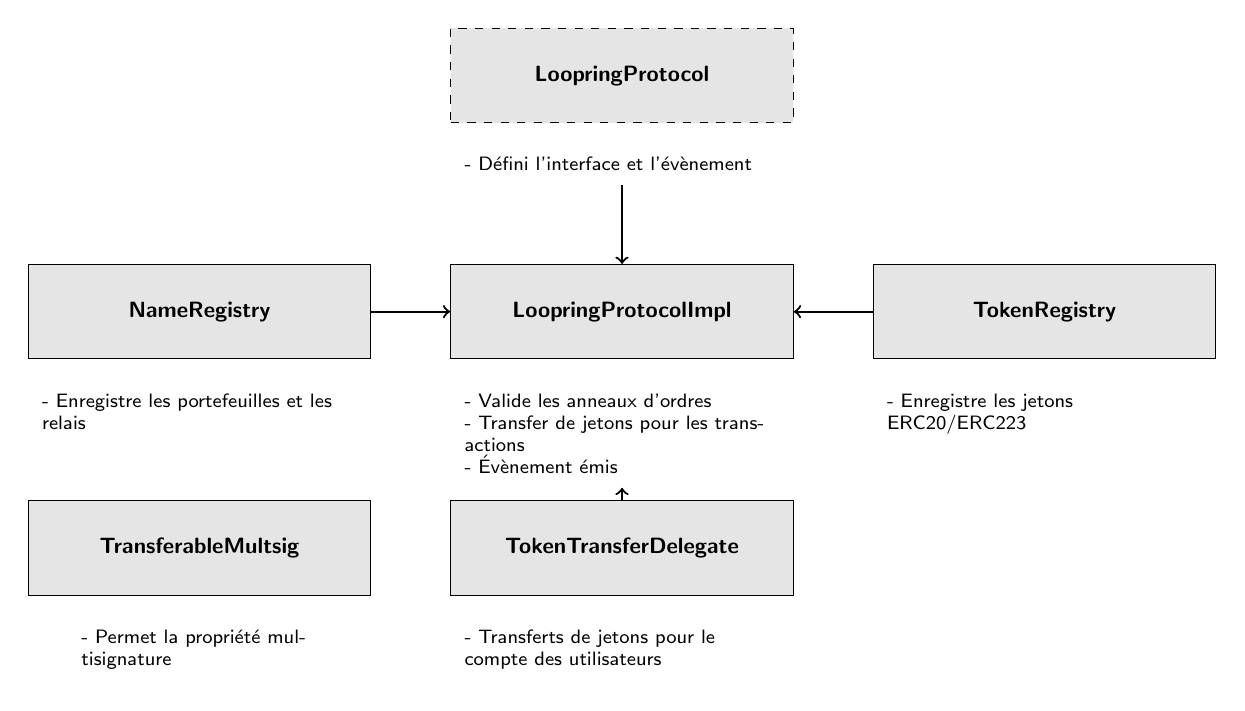
\begin{tikzpicture}
[node distance = 1cm, auto,font=\footnotesize,
% STYLES
every node/.style={node distance=3cm},
% The comment style is used to describe the characteristics of each force
comment/.style={rectangle, inner sep= 5pt, text width=4cm, node distance=0.25cm, font=\scriptsize\sffamily},
% The force style is used to draw the forces' name
force/.style={rectangle, draw, fill=black!10, inner sep=5pt, text width=4cm, text badly centered, minimum height=1.2cm, font=\bfseries\footnotesize\sffamily}] 

% Draw forces
\node [force] (impl) {LoopringProtocolImpl};
\node [force, dashed, above of=impl] (protocol_interface) {LoopringProtocol};
\node [force, left=1cm of impl] (nameregistry) {NameRegistry};
\node [force, right=1cm of impl] (tokenregistry) {TokenRegistry};
\node [force, below of=impl] (delegate) {TokenTransferDelegate};
\node [force, left=1cm of delegate] (multisig) {TransferableMultsig};

%%%%%%%%%%%%%%%
% Change data from here

% impl
\node [comment, below=0.25 of impl] (comment-impl) {- Valide les anneaux d'ordres\\
- Transfer de jetons pour les transactions\\
- Évènement émis};

% nameregistry
\node [comment, below=0.25cm of nameregistry]{- Enregistre les portefeuilles et les relais};

% protocol_interface
\node [comment, below=0.25 of protocol_interface](comment-interface) {- Défini l'interface et l'évènement};

% tokenregistry
\node [comment, below=0.25 of tokenregistry] {- Enregistre les jetons ERC20/ERC223};

% delegate
\node [comment, below=0.25 of delegate] {- Transferts de jetons pour le compte des utilisateurs};

% PUBLIC POLICIES
\node [comment, text width=3cm, below=0.25 of multisig] {- Permet la propriété multisignature};

%%%%%%%%%%%%%%%%

% Draw the links between forces
\path[->,thick] 
(comment-interface) edge (impl)
(nameregistry) edge (impl)
(tokenregistry) edge (impl)
(delegate) edge (comment-impl);

\end{tikzpicture} 
\caption{Contrats Intelligent}
\label{fig:smartcontracts}
\end{figurehere}
\end{center}

\subsection{Déploiement}

Les contrats intelligents suivants ont été déployés sur le réseau principal d'Éthereum :
\begin{itemize}
\item LRC: \verb|0xEF68e7C694F40c8202821eDF525dE3782458639f|
\item TokenRegistry: \verb|0xa21c1f2AE7f721aE77b1204A4f0811c642638da9|
\item TokenTransferDelegate: \verb|0xc787aE8D6560FB77B82F42CED8eD39f94961e304|
\item NameRegistry: \verb|0x0f3Dce8560a6010DE119396af005552B7983b7e7|
\item LoopringProtocolImpl: \verb|0xc80BbAb86cED62CF795619A357581FaF0cB46511|
\item TransferableMultsig: \verb|0x7421ad9C880eDF007a122f119AD12dEd5f7C123B|
\end{itemize}

\end{appendices}
\end{document}
